\documentclass{standalone}
\usepackage{pgfplots}
\begin{document}
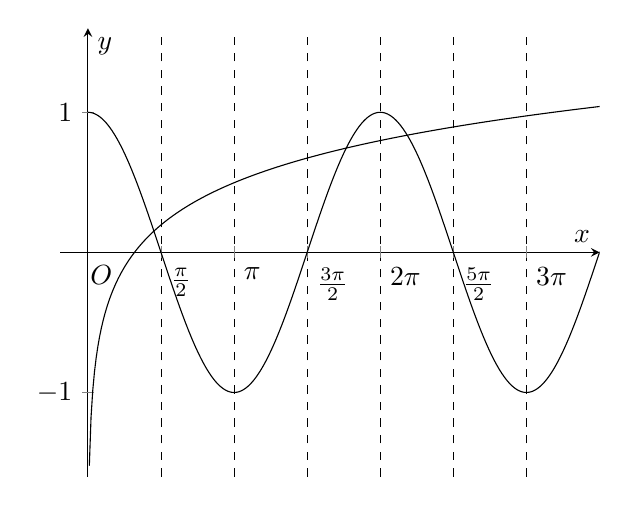
\begin{tikzpicture}
\begin{axis}
[
ymin=-1.6,ymax=1.6,
xmin=-0.6,xmax=11,
xtick=\empty,
ytick=\empty,
extra x ticks={1.5708, 3.14159, 4.71239, 6.28319, 7.85398, 9.42478},
extra x tick labels={$\frac{\pi}{2}$, $\pi$, $\frac{3\pi}{2}$, $2\pi$, $\frac{5\pi}{2}$, $3\pi$},
extra y ticks={-1, 1},
extra y tick labels={$-1$, $1$},
every extra x tick/.style={
    xticklabel style={anchor=north west},
    grid=major,
    major grid style={very thin,dashed,black}
},
axis lines = center,
xlabel=$x$,ylabel=$y$,
samples=200,
]
\addplot [black, domain=0:11, samples=300] {cos(deg(x))};
\addplot [black, domain=0.03:11, samples=300] {log10(x)};
\node at (axis cs:0.29, -0.16) {$O$} ;
\end{axis}
\end{tikzpicture}
\end{document}
